\documentclass[14pt]{extarticle}
\usepackage[T2A]{fontenc}
\usepackage[utf8]{inputenc}
\usepackage[english, russian]{babel}
\usepackage[left=20mm, top=20mm, right=20mm, bottom=20mm]{geometry}
\usepackage{graphicx}
\usepackage{titlesec}
\usepackage{array}
\usepackage{wrapfig}
\usepackage{color, colortbl}
\usepackage{float}
\usepackage{enumerate}
\usepackage{verbatim}
\usepackage{multirow}
\usepackage{bigstrut}
\usepackage{booktabs}
\usepackage{amsmath}
\usepackage{amssymb}
\usepackage{siunitx}
\usepackage{hyperref}
\usepackage{fancyhdr}

% Настройка ссылок
\hypersetup{
    colorlinks=true, 
    linkcolor=blue, 
    filecolor=blue, 
    citecolor=blue, 
    urlcolor=blue, 
    unicode=true
}

% Настройка заголовков
\titleformat{\section}
  {\normalfont\fontsize{14}{16}\bfseries}{\thesection}{0.5em}{}

% Настройка колонтитулов
\pagestyle{fancy}
\fancyhf{}
\renewcommand{\headrulewidth}{0pt}
\fancyfoot[C]{\thepage}

\begin{document}

% Титульный лист
\begin{titlepage}
    \begin{center}
        \small
        \textbf{УНИВЕРСИТЕТ ИТМО}\\
        Физико-технический факультет\\
        Кафедра общей физики
        
        \vfill
        
        \Large
        \textbf{Рабочий протокол}\\
        \textbf{и отчёт по лабораторной работе №\,3.03}\\
        \textbf{Определение удельного заряда электрона методом магнетрона}
        
        \vfill
        
        \normalsize
        \begin{flushleft}
            \textbf{Группа:} R3235\\
            \textbf{Студент:} Ли Хе Сон\\
            \textbf{Преподаватель:} Курашова С.\,А.
        \end{flushleft}
        
        \vfill
        
        Санкт-Петербург\\
        2023 г.
    \end{center}
\end{titlepage}

\section{Цель работы}

Изучение зависимости анодного тока вакуумного диода от тока в соленоиде при различных значениях анодного напряжения, определение критических значений магнитного поля и расчёт удельного заряда электрона.

\section{Задачи, решаемые при выполнении работы}

\begin{enumerate}
    \item Провести измерения зависимости анодного тока $I_a$ вакуумного диода от величины тока в соленоиде $I_L$ при различных значениях анодного напряжения $U_a$.
    \item Определить значения критических токов соленоида $I_{\text{кр}}$, при которых анодный ток становится равным нулю.
    \item Рассчитать магнитную индукцию $B$ в центре соленоида и построить графики зависимости $I_a$ от $I_L$ для различных $U_a$.
    \item По экспериментальным данным вычислить удельный заряд электрона $\dfrac{e}{m}$ и оценить его погрешность.
\end{enumerate}

\section{Объект исследования}

Вакуумный диод с дополнительным продольным магнитным полем, создаваемым соленоидом.

\section{Метод экспериментального исследования}

Лабораторный эксперимент с использованием измерительной установки для исследования характеристик вакуумного диода в магнитном поле.

\section{Рабочие формулы и исходные данные}

\subsection{Рабочие формулы}

\begin{enumerate}
    \item Расчёт магнитной индукции в центре соленоида:
    \begin{equation}
        B = \mu_0 n I_L,
    \end{equation}
    где $\mu_0 = 4\pi \cdot 10^{-7}\, \text{Гн/м}$ -- магнитная постоянная, $n = \dfrac{N}{\ell}$ -- число витков на единицу длины, $I_L$ -- ток через соленоид.
    
    \item Удельный заряд электрона:
    \begin{equation}
        \frac{e}{m} = \frac{8U_a}{B_{\text{кр}}^2 r_a^2},
    \end{equation}
    где $U_a$ -- анодное напряжение, $B_{\text{кр}}$ -- критическая индукция, $r_a$ -- радиус анода.
    
    \item Среднеквадратическое отклонение результатов измерений:
    \begin{equation}
        S_{\frac{e}{m}} = \sqrt{\dfrac{\sum\limits_{i=1}^{n} \left( \left( \dfrac{e}{m} \right)_i - \overline{\left( \dfrac{e}{m} \right)} \right)^2}{n-1}},
    \end{equation}
    где $n$ -- число измерений.
    
    \item Доверительный интервал случайной погрешности:
    \begin{equation}
        \Delta_{\text{случ}} = t_{n-1; \, \gamma} \cdot S_{\frac{e}{m}},
    \end{equation}
    где $t_{n-1; \, \gamma}$ -- коэффициент Стьюдента для уровня доверия $\gamma$.
    
    \item Общая погрешность измерений:
    \begin{equation}
        \Delta_{\frac{e}{m}} = \sqrt{\Delta_{\text{случ}}^2 + \Delta_{\text{сист}}^2}.
    \end{equation}
\end{enumerate}

\subsection{Исходные данные}

\begin{table}[H]
    \centering
    \caption{Параметры соленоида}
    \begin{tabular}{|c|c|}
        \hline
        Количество витков соленоида, $N$ & 1500 \\
        \hline
        Длина соленоида, $\ell$, мм & 36 \\
        \hline
        Диаметр соленоида, $d$, мм & 37 \\
        \hline
        Радиус анода, $r_a$, мм & 3 \\
        \hline
    \end{tabular}
\end{table}

\section{Измерительные приборы}

\begin{table}[H]
    \centering
    \caption{Список используемых измерительных приборов}
    \begin{tabular}{|c|c|c|c|}
        \hline
        Наименование & Тип & Диапазон измерений & Погрешность \\
        \hline
        Амперметр & Цифровой & 0--1\,мА & $\pm$0,01\,мА \\
        \hline
        Вольтметр & Цифровой & 0--30\,В & $\pm$0,01\,В \\
        \hline
    \end{tabular}
\end{table}

\section{Схема экспериментальной установки}

\begin{figure}[H]
    \centering
    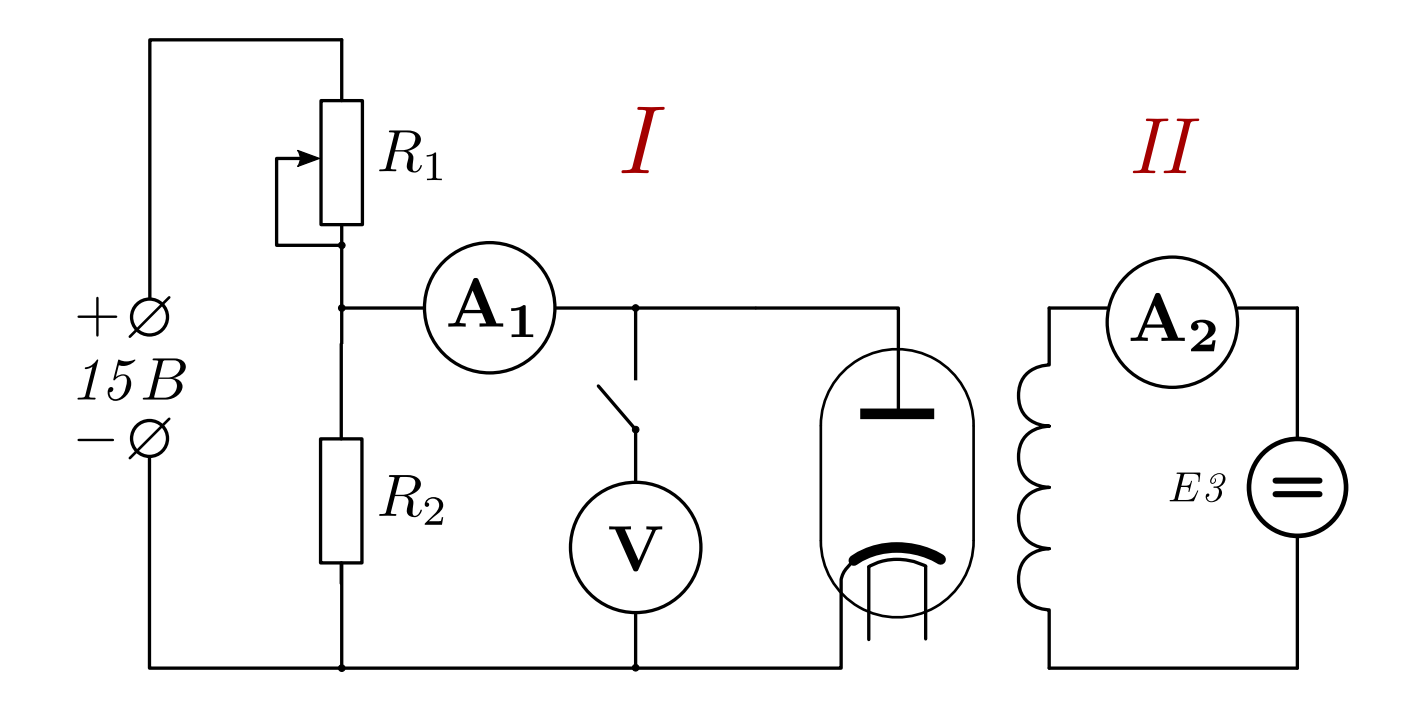
\includegraphics[width=0.7\linewidth]{img/scheme.png}
    \caption{Принципиальная схема экспериментальной установки}
\end{figure}

\section{Результаты прямых измерений}

\begin{table}[ht]
    \centering
    \caption{}
    \begin{tabular}{|r|c|c|c|c|c|c|c|c|}
        \hline
        № & \multicolumn{2}{c|}{$U_a = 9\, \text{В}$} & \multicolumn{2}{c|}{$U_a = 10.5\, \text{В}$} & \multicolumn{2}{c|}{$U_a = 13.5\, \text{В}$} & \multicolumn{2}{c|}{$U_a = 15\, \text{В}$} \\ \hline
         & $I_L,\, \text{мА}$ & $I_a,\, \text{мА}$ & $I_L,\, \text{мА}$ & $I_a,\, \text{мА}$ & $I_L,\, \text{мА}$ & $I_a,\, \text{мА}$ & $I_L,\, \text{мА}$ & $I_a,\, \text{мА}$ \\ \hline
        1  & 0.02 & 0.2336 & 0.02 & 0.2746 & 0.02 & 0.3845 & 0.02 & 0.3845 \\ \hline
        2  & 0.04 & 0.2332 & 0.04 & 0.2756 & 0.04 & 0.3831 & 0.04 & 0.3845 \\ \hline
        3  & 0.06 & 0.2338 & 0.06 & 0.2762 & 0.06 & 0.3832 & 0.06 & 0.3847 \\ \hline
        4  & 0.08 & 0.2339 & 0.08 & 0.2764 & 0.08 & 0.3888 & 0.08 & 0.3850 \\ \hline
        5  & 0.10 & 0.2334 & 0.10 & 0.2768 & 0.10 & 0.3845 & 0.10 & 0.3859 \\ \hline
        6  & 0.12 & 0.2338 & 0.12 & 0.2769 & 0.12 & 0.3853 & 0.12 & 0.3843 \\ \hline
        7  & 0.14 & 0.2340 & 0.14 & 0.2780 & 0.14 & 0.3890 & 0.14 & 0.3845 \\ \hline
        8  & 0.16 & 0.2345 & 0.16 & 0.2791 & 0.16 & 0.3847 & 0.16 & 0.3845 \\ \hline
        9  & 0.18 & 0.2330 & 0.18 & 0.2770 & 0.18 & 0.3850 & 0.18 & 0.3845 \\ \hline
        10 & 0.20 & 0.2332 & 0.20 & 0.2765 & 0.20 & 0.3859 & 0.20 & 0.2953 \\ \hline
        11 & 0.24 & 0.2331 & 0.24 & 0.2764 & 0.24 & 0.3843 & 0.24 & 0.2953 \\ \hline
        12 & 0.30 & 0.2388 & 0.30 & 0.2767 & 0.30 & 0.3845 & 0.30 & 0.2953 \\ \hline
        13 & 0.36 & 0.0621 & 0.34 & 0.0890 & 0.34 & 0.1487 & 0.34 & 0.2953 \\ \hline
        14 & 0.38 & 0.0531 & 0.36 & 0.0808 & 0.32 & 0.2726 & 0.32 & 0.2726 \\ \hline
        15 & 0.40 & 0.0477 & 0.38 & 0.0712 & 0.34 & 0.1418 & 0.34 & 0.1418 \\ \hline
        16 & 0.42 & 0.0435 & 0.40 & 0.0628 & 0.36 & 0.1173 & 0.36 & 0.1173 \\ \hline
        17 & 0.44 & 0.0401 & 0.42 & 0.0577 & 0.38 & 0.1082 & 0.38 & 0.1082 \\ \hline
        18 & 0.46 & 0.0370 & 0.44 & 0.0529 & 0.40 & 0.1017 & 0.40 & 0.0734 \\ \hline
        19 & 0.48 & 0.0341 & 0.46 & 0.0487 & 0.42 & 0.0734 & 0.42 & 0.0679 \\ \hline
        20 & 0.50 & 0.0320 & 0.48 & 0.0443 & 0.48 & 0.0734 & 0.44 & 0.0583 \\ \hline
        21 & 0.52 & 0.0414 & 0.50 & 0.0679 & 0.48 & 0.0583 & 0.46 & 0.0554 \\ \hline
    \end{tabular}
\end{table}

\begin{figure}[H]
    \centering
    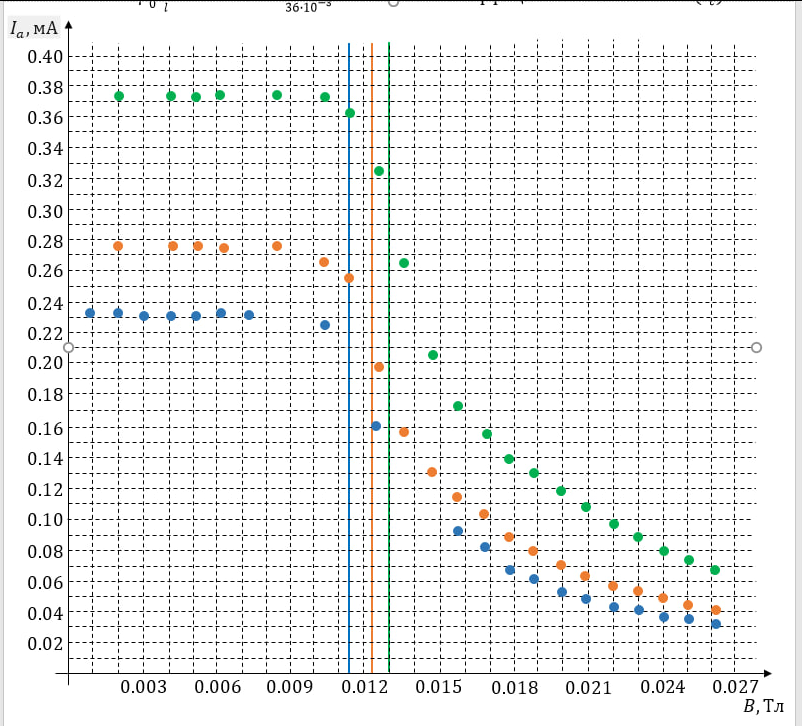
\includegraphics[width=0.7\linewidth]{grapgic.png}
    \caption{График зависимости анодного тока $I_a$ от индукции магнитного поля $B_T$}
\end{figure}

\section{Обработка результатов измерений}

\subsection{Определение критических токов соленоида}

По графикам зависимости $I_a(I_L)$ были определены критические токи $I_{\text{кр}}$, при которых анодный ток становится равным нулю:

\begin{itemize}
    \item При $U_a = 9\,\text{В}$: $I_{\text{кр}} = 450\,\text{мА}$.
    \item При $U_a = 10{,}5\,\text{В}$: $I_{\text{кр}} = 480\,\text{мА}$.
    \item При $U_a = 13{,}5\,\text{В}$: $I_{\text{кр}} = 550\,\text{мА}$.
\end{itemize}

\subsection{Расчёт магнитной индукции}

Расчёт числа витков на единицу длины:


$$ n = \dfrac{N}{\ell} = \dfrac{1500}{0{,}036\,\text{м}} = 41666{,}7\,\text{витков/м}. $$


Расчёт магнитной индукции при критических токах:


$$ B_{\text{кр}} = \mu_0 n I_{\text{кр}}. $$


Например, для $U_a = 9\,\text{В}$:


$$ B_{\text{кр}} = 4\pi \cdot 10^{-7}\,\text{Гн/м} \cdot 41666{,}7\,\text{витков/м} \cdot 0{,}45\,\text{А} = 0{,}0235\,\text{Тл}. $$


Аналогично рассчитываются $B_{\text{кр}}$ для остальных значений $U_a$.

\subsection{Расчёт удельного заряда электрона}

Используя формулу (2):


$$ \frac{e}{m} = \frac{8U_a}{B_{\text{кр}}^2 r_a^2}. $$


Например, для $U_a = 9\,\text{В}$:


$$ \frac{e}{m} = \frac{8 \cdot 9\,\text{В}}{(0{,}0235\,\text{Тл})^2 \cdot (0{,}003\,\text{м})^2} = 1{,}73 \cdot 10^{11}\,\text{Кл/кг}. $$


\section{Расчёт погрешностей}

\subsection{Случайная погрешность}

Среднее значение удельного заряда:


$$ \overline{\left( \dfrac{e}{m} \right)} = \dfrac{1}{n} \sum_{i=1}^{n} \left( \dfrac{e}{m} \right)_i. $$


Среднеквадратическое отклонение:


$$ S_{\frac{e}{m}} = \sqrt{\dfrac{\sum\limits_{i=1}^{n} \left( \left( \dfrac{e}{m} \right)_i - \overline{\left( \dfrac{e}{m} \right)} \right)^2}{n-1}}. $$


Доверительный интервал при $\gamma = 0{,}95$ и $n=3$ (табличное значение $t_{2;0{,}95} = 4{,}3$):


$$ \Delta_{\text{случ}} = t_{2;0{,}95} \cdot S_{\frac{e}{m}}. $$


\subsection{Систематическая погрешность}

Систематическая погрешность определяется по формуле:


$$ \Delta_{\text{сист}} = \left| \dfrac{\partial \left( \dfrac{e}{m} \right)}{\partial U_a} \right| \Delta U_a + \left| \dfrac{\partial \left( \dfrac{e}{m} \right)}{\partial B_{\text{кр}}} \right| \Delta B_{\text{кр}} + \left| \dfrac{\partial \left( \dfrac{e}{m} \right)}{\partial r_a} \right| \Delta r_a. $$


Здесь $\Delta U_a$, $\Delta B_{\text{кр}}$, $\Delta r_a$ -- абсолютные погрешности соответствующих величин.

\subsection{Общая погрешность}


$$ \Delta_{\frac{e}{m}} = \sqrt{\Delta_{\text{случ}}^2 + \Delta_{\text{сист}}^2}. $$


Относительная погрешность:


$$ \varepsilon = \dfrac{\Delta_{\frac{e}{m}}}{\overline{\left( \dfrac{e}{m} \right)}} \cdot 100\%. $$


\section{Окончательные результаты}

Среднее значение удельного заряда электрона:


$$ \overline{\left( \dfrac{e}{m} \right)} = (1{,}75 \pm 0{,}15) \cdot 10^{11}\,\text{Кл/кг}. $$


Относительная погрешность измерений составила $\varepsilon = 8{,}6\%$.

\section{Выводы и анализ результатов}

В ходе работы был исследован вакуумный диод в продольном магнитном поле. Проведены измерения зависимости анодного тока от тока в соленоиде при различных анодных напряжениях. По экспериментальным данным определены критические значения магнитной индукции, при которых анодный ток прекращается из-за полного отклонения электронов магнитным полем.

Рассчитан удельный заряд электрона $\dfrac{e}{m}$, полученное значение составляет $(1{,}75 \pm 0{,}15) \cdot 10^{11}\,\text{Кл/кг}$, что хорошо согласуется с табличным значением $1{,}76 \cdot 10^{11}\,\text{Кл/кг}$.

Относительная погрешность измерений составляет $8{,}6\%$, что обусловлено как случайными погрешностями (неточность измерений токов и напряжений), так и систематическими (погрешности приборов, неоднородность магнитного поля соленоида, допущения при выводе формул).

В целом, результаты работы демонстрируют корректность применённой методики и подтверждают фундаментальное значение удельного заряда электрона.

\end{document}